\chapter{Results and Discussions}
\label{results}

%-include prelim results from testbed

This chapter presents the evaluation of MCRP. The experiment set up for Cooja simulation and FlockLab \cite{flocklab} testbed are explained below. In Cooja simulation, interference is introduced. MCRP is evaluated using an end-to-end packet delivery performance metric. The results from the experiments are presented and discussed. 

%The testbed provides the ability to validate performance in real wireless channel environments. 
%However, relying solely on testbed results complicates the task of examining the network's behaviour and diagnosing the root causes of performance degradations. 
%For this purpose, while simulators lack the realism of testbeds, we leverage their ability to provide repeatability and full control over the parameter space. 
%Furthermore, unlike a testbed setup, which is by necessity confined both in time and in space, a simulation can be made arbitrary complex (introduce interference**. 
%Although simulators cannot be expected to fully mimic the behaviour of real wireless channels, they are effective in discovering the root causes underlying the performance degradations caused from implementation-specific design choices \cite{beyondInteroperability}.

\section{Experimental Setup}
MCRP is evaluated in Cooja simulated environment and FlockLab testbed. In Cooja simulation, an interference model is used as simulation allows full control over the test environment and the experiments are repeatable. Although the interference model does not fully mimic the behaviour of real world interference, it enables MCRP performance to be tested in various conditions when the channel performance degraded. Unlike simulation, testbed provides the ability to validate MCRP performance in the real wireless channel environments. However, the network's behaviour are complicated to examine, thus, comparing the testbed result with simulation results give a better understanding of the performance. 

%We evaluate the protocol in Cooja simulated environment and FlockLab \cite{flocklab} testbed.

%We use an end-to-end packet delivery performance metric to evaluate MCRP. The transmission success rate is calculated from the sender to the receiver over multiple hops. 

%The simulations are repeated ten times. In all plots, the mean value of the ten simulations is plotted with error bars corresponding to one standard deviation in either deviation to give a measure of repeatability. The plots are of the proportion of received packets (from 0\% to 100\%) against time where the loss is measured over the previous time period.  The x-value is shifted slightly left and right to prevent error bars overlapping.

\subsection{Simulation}
MCRP is evaluated in the Cooja simulated environment with emulation of TMote sky nodes that feature the CC2420 transceiver, a 802.15.4 radio. The nodes run on IPv6, using UDP with standard RPL and 6LoWPAN protocols. The network consists of 31 nodes which are used to run the simulation where one node is used as the border router node, 16 interference nodes, and 14 duty cycled nodes that act as UDP clients to send packets to LPBR spanning over 20-30 metres between each node. RPL border router is used as LPBR in order to move most processing decisions on a PC as it has more RAM and better processing capabilities than a sensor. TelosB has limited RAM and ROM of 10K bytes and 48K bytes of flash memory \cite{telosb-datasheet}. By using a border router, this allows channel changing to be decided in real time without draining the memory and battery on a sensor. The border router also acts as the root of the tree.
%We evaluate the protocol in the Cooja simulated environment with emulation of TMote sky nodes that feature the CC2420 transceiver, a 802.15.4 radio and on Flocklab \cite{flocklab} testbed. The nodes run on IPv6, using UDP with standard RPL and 6LoWPAN protocols. In Cooja, the network consists of 31 nodes which are used to run the simulation where we have 1 border router node, 16 interference nodes, and 14 duty cycled nodes that act as UDP clients to send packets to LPBR spanning over 20-30 metres between each node. On testbed, the network consists of 26 nodes; 1 border router node and 25 duty cycled nodes. The nodes are distributed in offices, hallways and storerooms across one floor in an office building. We do not introduce interference nodes as the testbed has external interference from the surrounding (e.g. from the co-located Wi-Fi or limited connectivity) to see the effect on MCRP. The link qualities estimation information of the tesbed is displayed on the Flocklab website. The link qualities and routing change throughout the day as the noise level on all channels and frequency bands are tested during testbed idle times. RPL border router is used as LPBR in order to move most processing decisions on a PC as it has more RAM and better processing capabilities than a sensor. TelosB has limited RAM and ROM of 10K bytes and 48K bytes of flash memory \cite{telosb-datasheet}. By using a border router, this allows channel changing to be decided in real time without draining the memory and battery on a sensor. The border router also acts as the root of the tree.

\begin{figure}
\centering
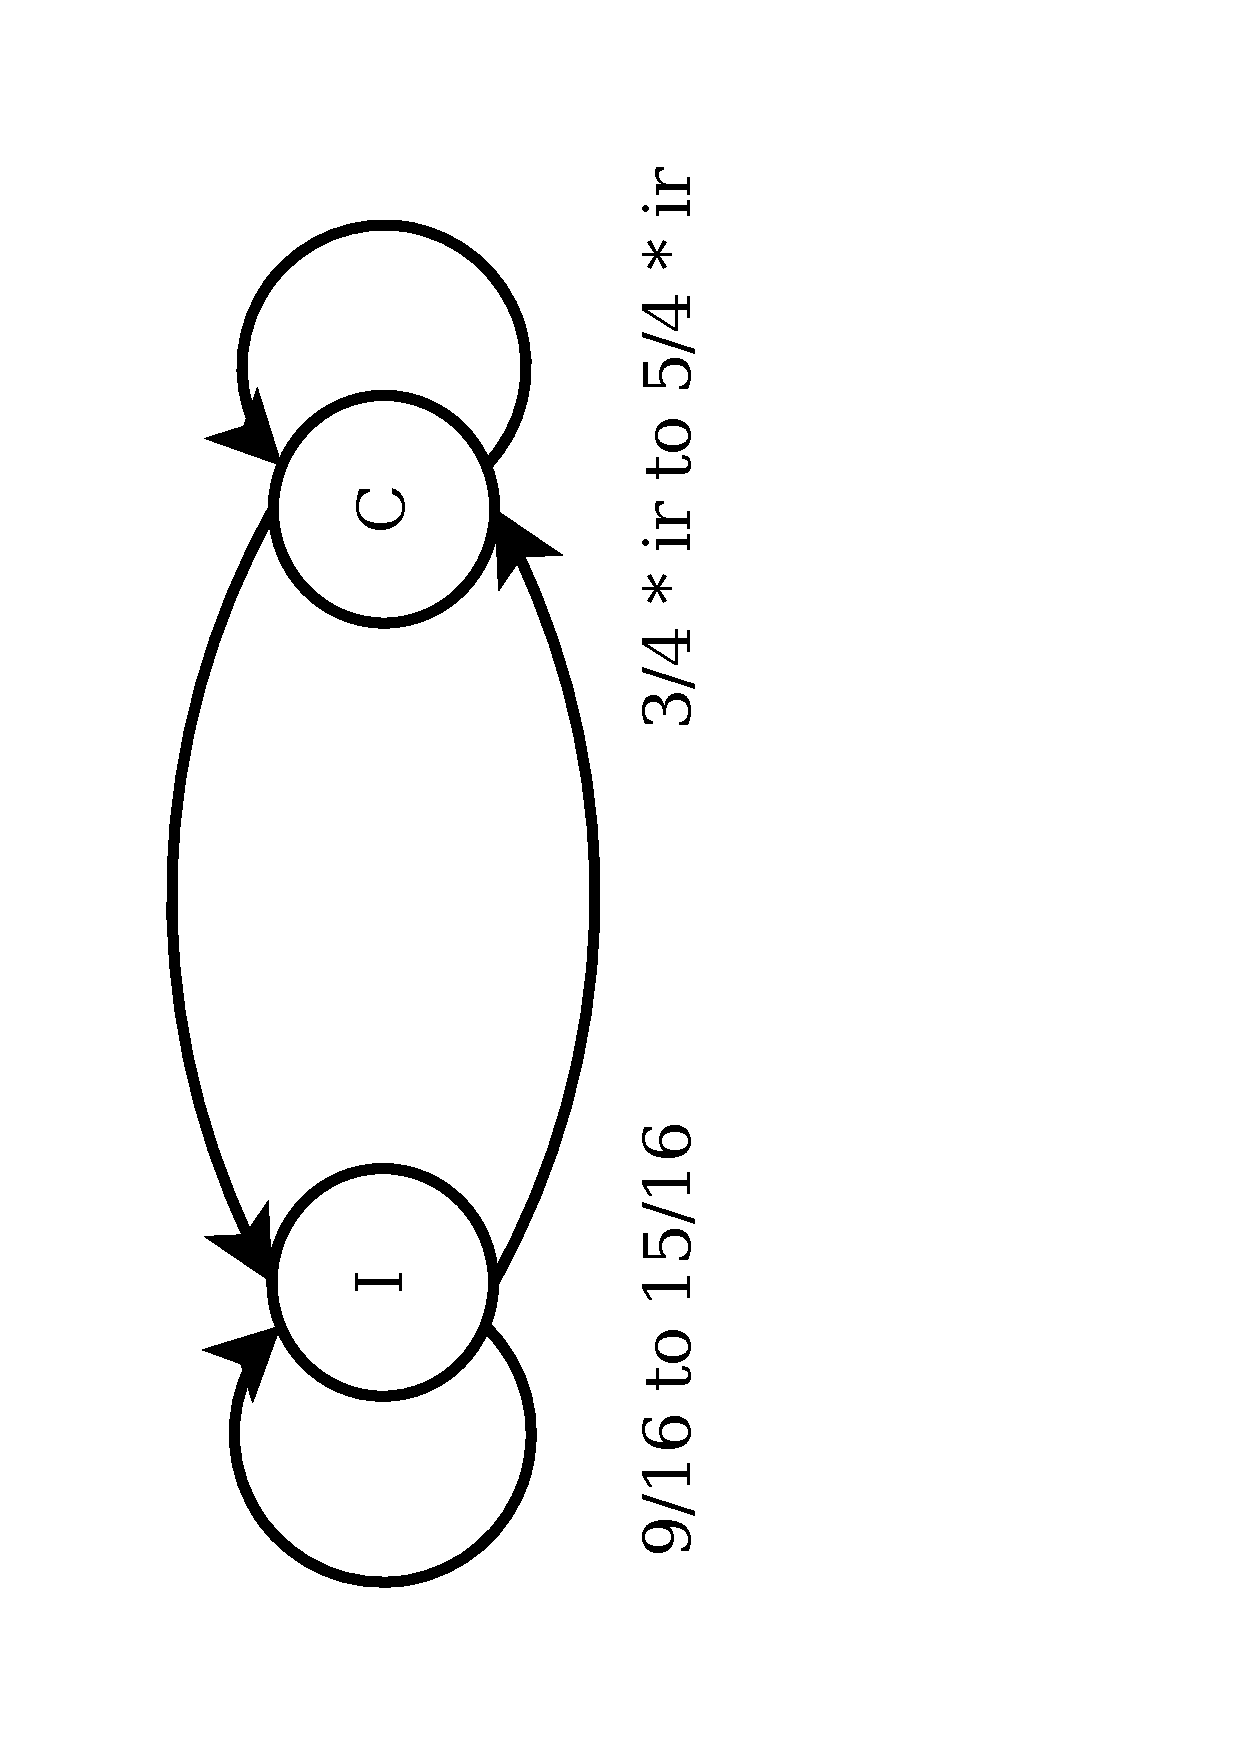
\includegraphics[trim=2cm 2cm 8cm 2cm, clip=true, totalheight=0.33\textheight, angle=270]{interferenceModel.pdf}
\caption{Low power border router}
\label{fig_interferenceModel}
\end{figure}

A controlled interference node that generates semi-periodic bursty interference is simulated to resemble a simplified Wi-Fi or Bluetooth transmitter on several channels at random. The interference model proposed in \cite{interferenceModel} is used in the simulation. The interference has two states, a clear state and an interference state. 
In the interference state, the interference node generates packets for a time that is uniformly distributed between $9/16$ seconds and $15/16$ seconds. In the clear state the interferer produces no packets and stays in this state for between $3/4 * \emph{clear\textunderscore time}$ and $5/4 * \emph{clear\textunderscore time}$ where \emph{clear\textunderscore time} refers to the rate of interference. The model is illustrated in Figure \ref{fig_interferenceModel}.
Multiple channels interference is used in the simulation to show the hypothesis that MCRP can help avoid interference. The scenario that is considered is where ContikiMAC with RPL system is subject to interference on its channel after set up has successfully completed so the RPL set up is allowed to complete before interference begins.

%We use an end-to-end packet delivery performance metric to evaluate MCRP. The transmission success rate is calculated from the sender to the receiver over multiple hops. 

The protocol performance in loss over time in the presence of interference is observed. Two multiple channels interference scenarios are considered; (1) extreme and no interference rate on 8 channels each and (2) extreme, moderate, mild and no interference rate on 4 channels each. The interference channels are randomly chosen from the available 16 channels and the same interference channels and rates are used throughout the experiments. However, channel 26 is kept clear from interference in order to ensure RPL set up is unaffected. In scenario 1, the interference rates are fixed to extreme and no interference to observe the effect it has on the channel changing decisions. In scenario 2, the interference rates are vary to observe how MCRP copes in deciding a channel when there is more interference than scenario 1 but with less interference intensity. 

The simulation runs for a duration of 45-60 minutes to send 210-560 packets. When the nodes are switched on for the first time, all nodes are initialised to channel 26, the default channel for Contiki MAC layer. RPL is allowed five minutes to set up (which is ample time). RPL topology is formed in a minute. The simulation waits for another five minutes to allow trickle timer to double the interval length so that RPL control messages are not being sent frequently. The multichannel protocol is then runs for 25 minutes. In the 15 nodes simulation, the protocol takes 20-25 minutes to run the channel change set up. Another 5 minutes wait time is allowed if retransmissions happen. 
In a single channel simulation, all the nodes are changed to channel 22 after 5 minutes of RPL set up time. This allows RPL to have enough time to discover all nodes to form an optimised topology. The topology formation does not form completely if the interference node interferes from the beginning. The interference node starts sending packets to interfere after 3 minutes the system is switched on so that the interference channel is involve in the channel changes decision. It is proven that the protocol tries to avoid changing to the interference channel through time out and probing failures. After 30 minutes, the client nodes will send a normal packet periodically every 30-60 seconds to LPBR. This is done in order to avoid collision of the nodes sending at the same time. 

%The simulations are repeated ten times. In all plots, the mean value of the ten simulations is plotted with error bars corresponding to one standard deviation in either deviation to give a measure of repeatability. The plots are of the proportion of received packets (from 0\% to 100\%) against time where the loss is measured over the previous time period.  The x-value is shifted slightly left and right to prevent error bars overlapping.

\subsection{Testbed}

\begin{figure}
\centering
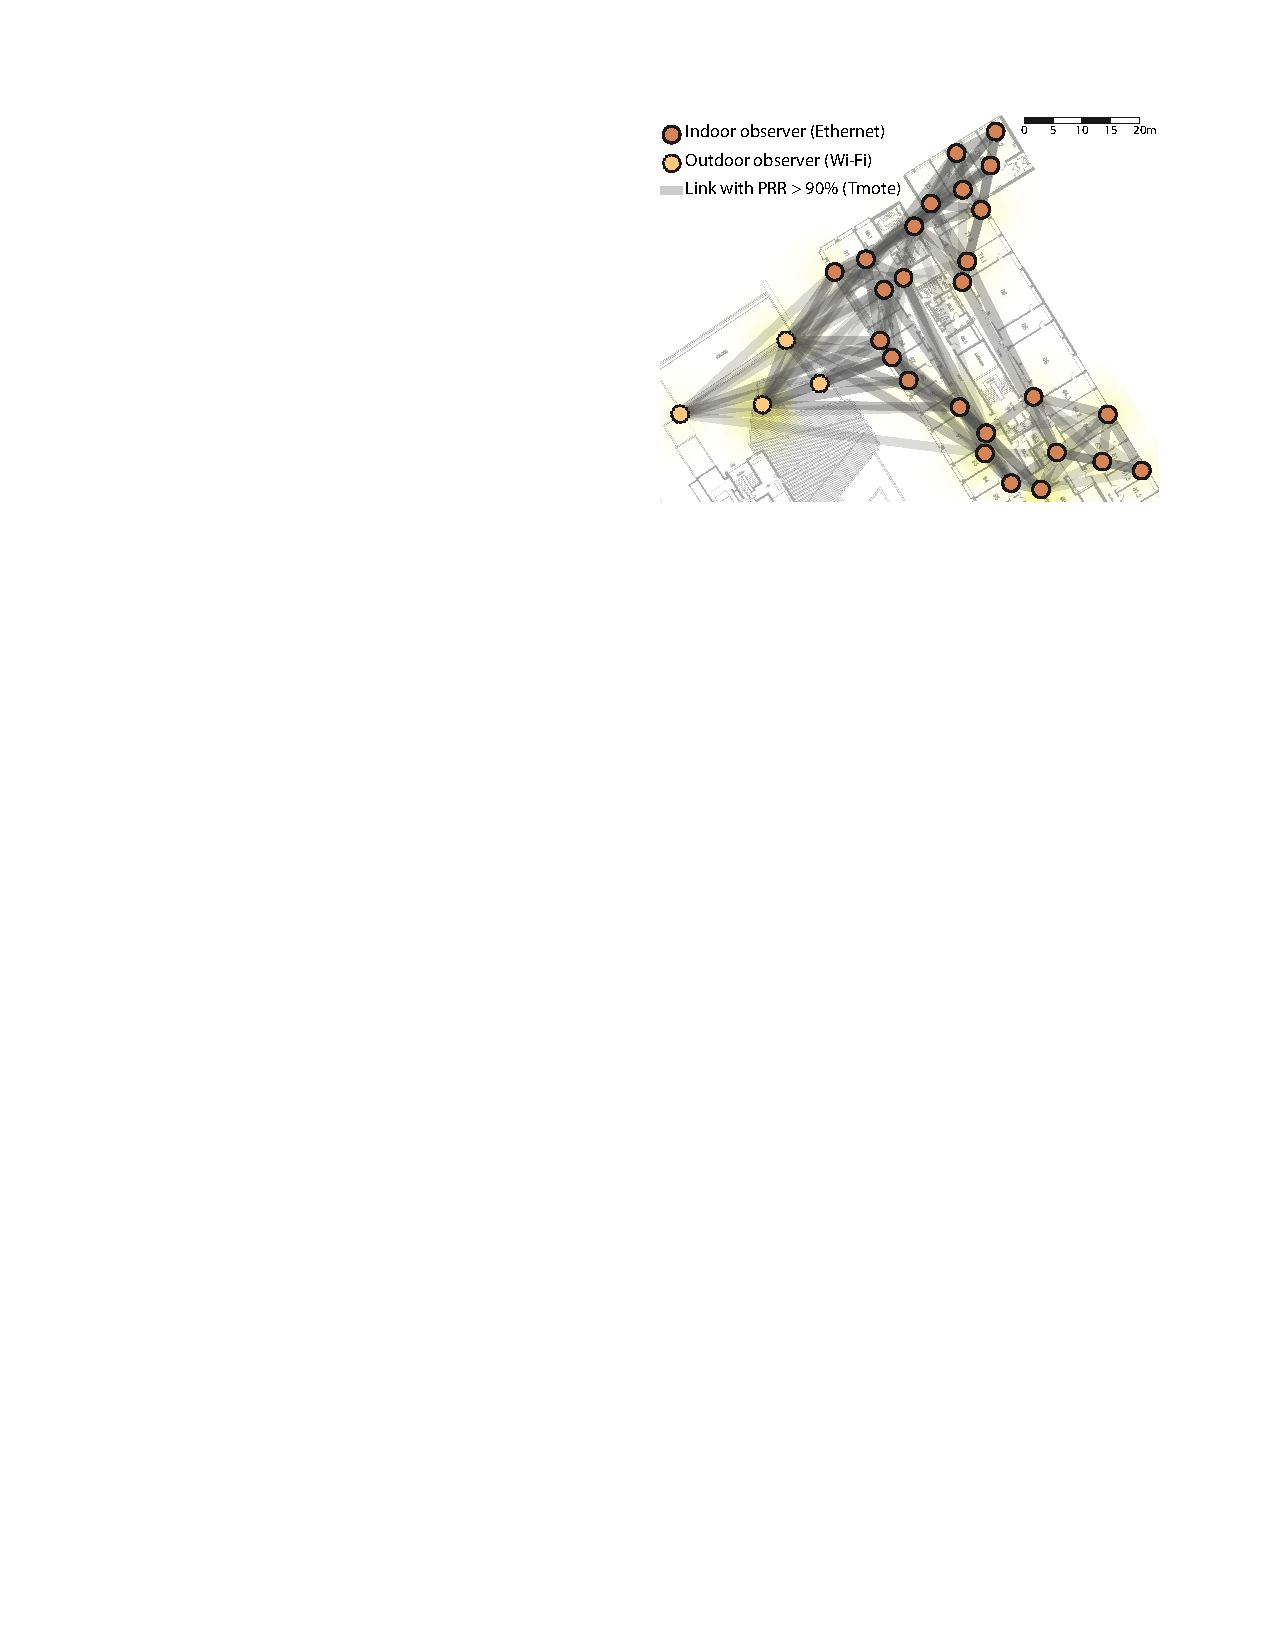
\includegraphics[trim=0cm 0cm 0cm 0cm, clip=true, totalheight=0.33\textheight]
{flocklabLayout.pdf}
\caption{Layout of FlockLab deployment}
\label{fig_flocklab}
\end{figure}

Similar to the simulation settings, the nodes run on IPv6, using UDP with standard RPL and 6LoWPAN protocols. The network consists of 26 nodes; 1 border router node and 25 duty cycled nodes as shown in Figure \ref{fig_flocklab} where the grey lines represent the link qualities between nodes and yellow gradient is the noise. The indoor nodes are distributed in offices, hallways and storerooms across one floor in an office building. Unlike in simulation, interference nodes are not added as the testbed has external interference from the surrounding (e.g. from the co-located Wi-Fi or limited connectivity) to see the effect on MCRP. The link qualities estimation information of the testbed is displayed on the FlockLab website. The link qualities and routing change throughout the day as the noise level on all channels and frequency bands are tested during testbed idle times.

As the channel condition in the testbed is beyond control, the experiment runs for a longer time period than the simulation. The testbed experiment is in the preliminary stage. The testbed is run for a duration of 4 hours to send up to 1250 packets depending on the availability of the nodes. The nodes are not switched on at the same time, thus RPL is allowed ten minutes to set up. MCRP is then run for 2 hours where the channel changes are done much slower than in the simulation as the channel condition is unknown, thus the number of retransmissions and collisions increases. The nodes wait for the normal incoming packet if the channel change processes finish early.

%///CHANGE We run the simulation for a duration of 45-60 minutes to send 210-560 packets. When the nodes are switched on for the first time, all nodes are initialised to channel 26, the default channel for Contiki MAC layer. RPL is allowed five minutes to set up (which is ample time). RPL topology is formed in a minute. We wait for another five minutes to allow trickle timer to double the interval length so that RPL control messages are not being sent frequently. We then let our multichannel protocol runs for 25 minutes. In our 15 nodes simulation, our protocol takes 20-25 minutes to run the channel change set up. We allow another 5 minutes wait time if retransmissions happen. 

\section{Evaluation}
The performance of MCRP is compared against the standard ContikiMAC with RPL. MCRP is analysed using an end-to-end packet delivery performance metric. The transmission success rate is calculated from the sender to the receiver over multiple hops. 

%We use an end-to-end packet delivery performance metric to evaluate MCRP. 

The simulations are repeated ten times. In all plots, the mean value of the ten simulations is plotted with error bars corresponding to one standard deviation in either deviation to give a measure of repeatability. The plots are of the proportion of received packets (from 0\% to 100\%) against time where the loss is measured over the previous time period.  The x-value is shifted slightly left and right to prevent error bars overlapping.

\subsection{Packet Loss Rates}
The performance obtained in ContikiMAC with RPL (single channel) is compared with MCRP in terms of packet loss rate.
As described previously, levels of interference used (referred to as \emph{clear\textunderscore time} in \cite{interferenceModel}) vary between 100\% (no interference), 75\% (mild), 50\% (moderate) and 25\% (extreme) where the percentage is the ratio of the time the channel is clear for transmission.  All of the tests have a common format: the RPL procedure is allowed to set up without interference in order not to bias subsequent tests.
Then the interferers begin to operate with a constant level (none, mild, moderate or extreme).

\begin{figure}
\centering
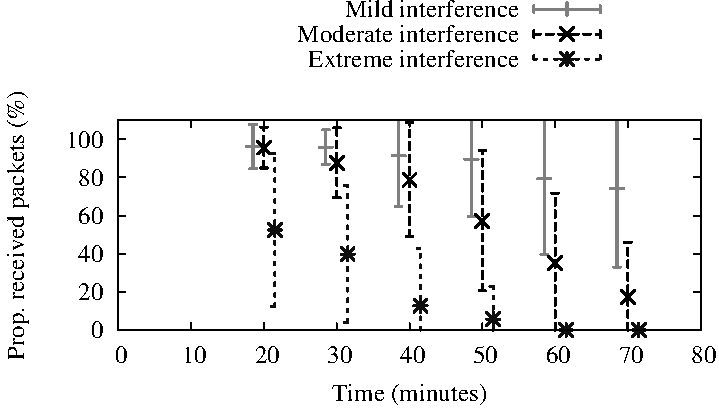
\includegraphics[width=0.78\textwidth]{single_channel.pdf}
\caption{Level of packet loss for mild, moderate and extreme interference levels using single channel}
\label{fig:interference}
\end{figure}

Figure \ref{fig:interference} shows the results in simulation for ContikiMAC with RPL protocol. It can be seen that the level of packet loss varies considerably between experiments (the error bars are always large). It can also be seen that even for mild interference there is considerable loss and this gets worse as time proceeds. In the extreme interference case the loss always goes up until no packets are received. For mild interference the system evolves until it is losing around 20\% of packets but this can increase.

The results from the single channel with interference is compared with the multichannel with the same interference rate of 75\% (mild), 50\% (moderate) and 25\% (extreme). The test is done to evaluate MCRP behaviour in different interference rate and to compare the result with a single channel case. 

\begin{figure}
\centering
\subfigure[Mild Interference]{\label{fig:mild}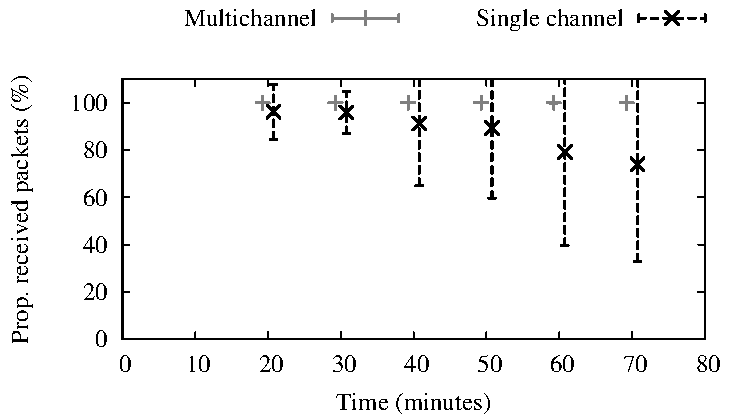
\includegraphics[width=0.78\textwidth]{experiments/mild.pdf}}                
\subfigure[Moderate Interference]{\label{fig:mod}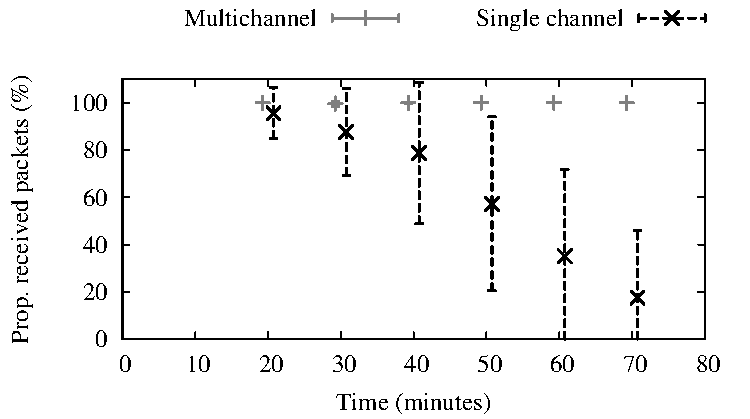
\includegraphics[width=0.78\textwidth]{experiments/moderate.pdf}}
\subfigure[Extreme Interference]{\label{fig:extreme}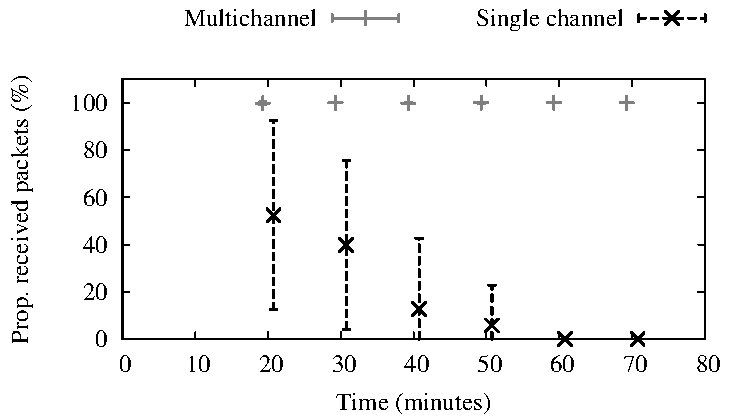
\includegraphics[width=0.78\textwidth]{experiments/extreme.pdf}}
\caption{Results of Multichannel RPL and a single channel RPL on different interference rate.}
\label{fig:sminterference}
\end{figure}

Figure \ref{fig:sminterference} shows the averaged results from ten runs that were done. It can be observed that during high and moderate interference, if LPBR tries to send a channel change value that is the same channel as the interference, the request will either timed out or if it succeeds, the probing messages received are less than a threshold that allows for the node to change its listening channel to the new channel. This is as expected as MCRP checks the channel each time before deciding on the new channel to avoid interference channel. By doing this, it ensure that the node's listening channel is a good channel. This enable the use of all available channels without blacklisting any channel until it is sure that it is a bad channel through the probing process. The channel quality table is built at the LPBR that over time can be used to learn good and bad channels based on several probing processes. MCRP avoids the interference channel which as a result, resulted in less loss than in a single channel case. 

In the single channel, the node does not have enough time to recover from the interference to retransmit and drops all packets. Figure \ref{fig:extreme} shows that there are more packets drop over time and it stops receiving packets as it doesn't have enough buffer to store the incoming packet and the channel becomes congested. However, as the interference rate increases (less interference), the single channel performance improves as it has more time to recover.

In the mild interference case, all probing messages are received even though there is interference in that channel. This means that the channel can be used for transmission. As the interference rate is mild, all packets are received. This is also the case with a single channel. The interference does not affect the transmissions as the interference is not frequent enough. The node has enough time to recover from the interference through retransmissions. However, the interference would slightly effect the packet transmission over time. The channel change processes should run periodically to avoid this from happening.

\begin{figure}
\centering
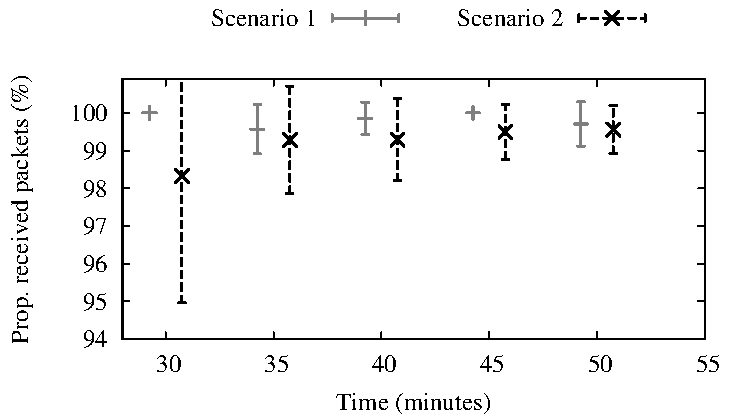
\includegraphics[width=0.78\textwidth]{multi_channel.pdf}
\caption{Level of packet loss for scenario 1 and scenario 2 using multi channel}
\label{fig:multi_interference}
\end{figure}

%\begin{figure}
%\centering
%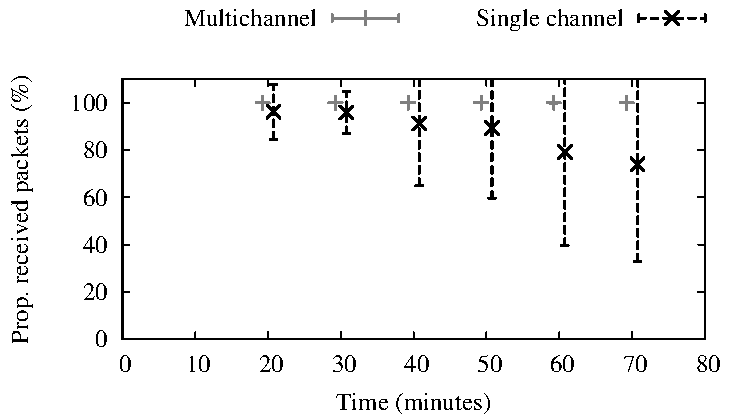
\includegraphics[width=0.78\textwidth]{experiments/mild.pdf}
%\caption{Mild interference on MCRP and a single channel}
%\label{fig:mild}
%\end{figure}

%\begin{figure}
%\centering
%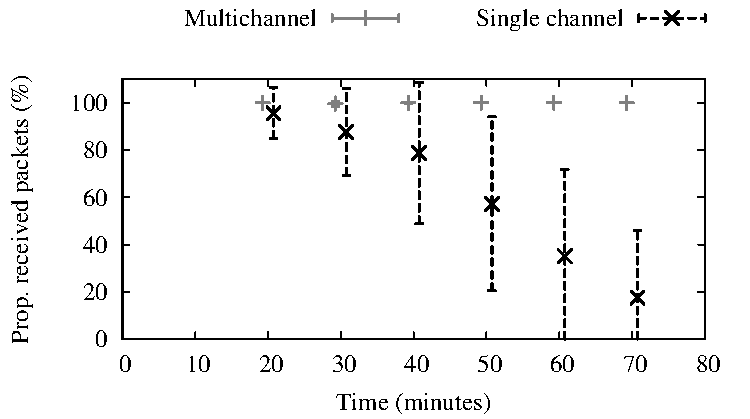
\includegraphics[width=0.78\textwidth]{experiments/moderate.pdf}
%\caption{Moderate interference on MCRP and a single channel}
%\label{fig:moderate}
%\end{figure}

%\begin{figure}
%\centering
%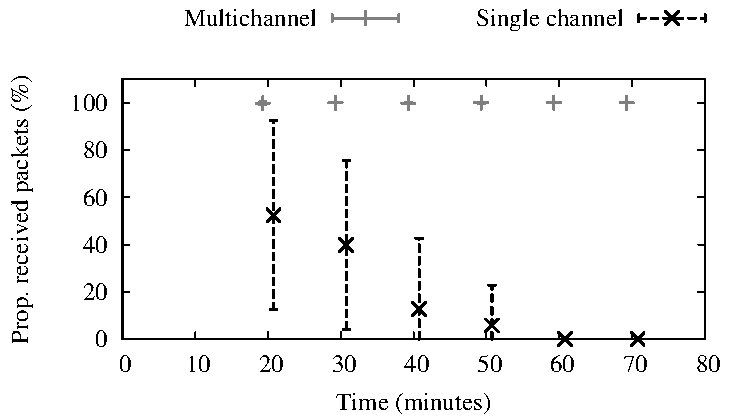
\includegraphics[width=0.78\textwidth]{experiments/extreme.pdf}
%\caption{Extreme interference on MCRP and a single channel}
%\label{fig:extreme}
%\end{figure}

To further evaluate MCRP capabilities to cope with interference from many sources, thus channels, two interference scenarios are considered.
In scenario 1 half the channels (including the original channel) have no
interference at all and half the channels have extreme interference.
In scenario 2, four channels (including the original channel) have no
interference, four have mild, four moderate and four extreme interference.
Figure \ref{fig:multi_interference} shows multi channel results for these
two scenarios. In scenario 1 the protocol performs extremely well, the packet loss is near zero and the protocol successfully detects channels with interference.
Scenario 2 has similar results as in scenario 1. The protocol does well at reducing the effects of interference and could detect moderate and mild interference.

%/////////TESTBED RESULT!
\begin{figure}
\centering
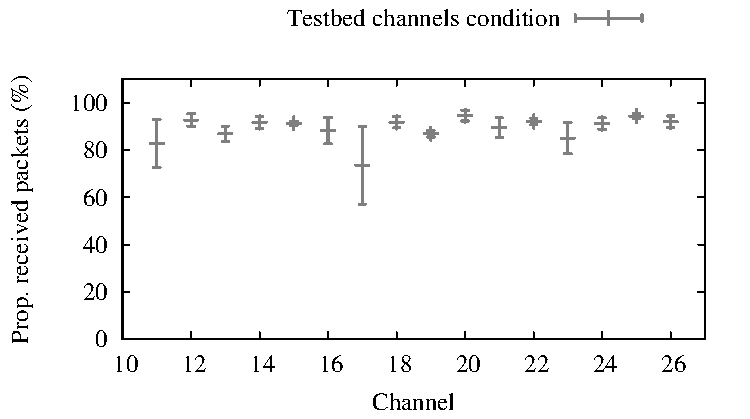
\includegraphics[width=0.78\textwidth]{experiments/chCondition.pdf}
\caption{Level of packet loss on testbed for different channels}
\label{fig:chCondition_testbed}
\end{figure}

In the testbed case, the conditions for all channels are looked into to have a better idea of the variation in interference. The channels are tested on all channels for three different days. Figure \ref{fig:chCondition_testbed} shows that the interference on the testbed varies for different channels on different days. However, it shows high receiving rate of 50\%-90\% in general.

%GRAPH OF TESTBED CH CONDITION (SEND TO LPBR) 

%GRAPH OF PKT LOSS FOR ALL CH PER NODE
%GRAPH OF MCRP

\begin{figure}
\centering
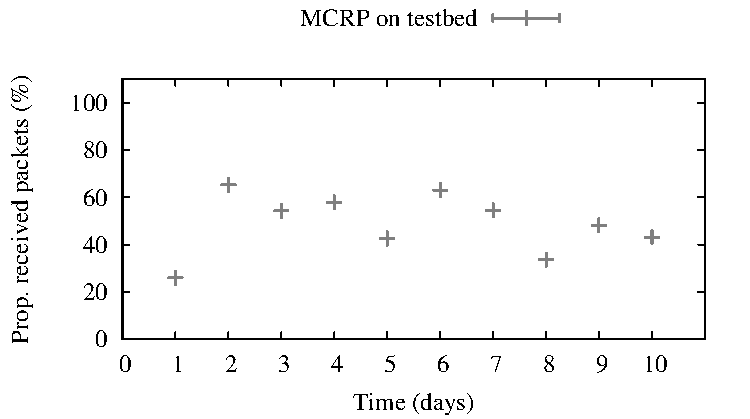
\includegraphics[width=0.78\textwidth]{experiments/mct.pdf}
\caption{Level of packet loss on testbed using multi channel}
\label{fig:mcrp_testbed}
\end{figure}

Figure \ref{fig:mcrp_testbed} shows the results from ten runs and the average that were done on different days. It can be observed that the results vary and multi channel give unstable results. On average, 50\%-60\% of packets are received at the LPBR. There are a few reasons for this low receiving packet values. As explained in Section \ref{bufmgmt}, the incoming and outgoing packets are kept in the same buffer. When the channel is busy the outgoing and incoming packets will fill up the buffer which results in new packet to be dropped. The dropped packets might be the important packets that decide or confirm the new channel. This results in sending in incorrect channel. The node will tries to send until it receives the link layer acknowledgement or time out which as a result, blocks the channel during its sending period by making the channel busy to be used by other node of the same channel. Another option to overcome this problem is by enabling RPL DIO on all channel so that the lost nodes can be recovered and updated with the correct channel each time the control message is sent. RPL DIO control message is sent to the neighbouring nodes according to the Trickle timer as explained in Section \ref{routingProtocols}.

%-buffer overflow (don't know the correct neighbour channel)
%-change channel from LPBR not receive - still in the default channel
%-packet that indicate change/not change not receive, thus node sends on the wrong channel (should consider send RPL DIO on all channel to recover lost nodes - DIS no being resent)

As the environment vary, it is not possible to replicate the same experiment as the topology might have changed depending on the RPL ETX value at each run. The nodes are possibly to take different routes to send the packet than in previous experiment.

In MiCMAC \cite{micmac}, it is stated that MiCMAC has a transmission success rate of 99\% when using four channels. However, when more than four channels are used (8 or 16 channels), MiCMAC performance degrades to approximately 88\% (16 channels) due to interference channels. The interference model that MiCMAC uses is different than in this experiment. They compare the result with Chrysso where Chrysso has a transmission success rate of approximately 88\% for 4 and 8 channels and suffers greatly in the case of 16 channels with 60\% success rate.
MCRP on the other hand, shows greatly reduced loss rate with any number of channels at approximately 99\%.

\subsection{Setup Overhead}
Obviously the system of changing channels and probing to see if a channel is free of interference introduces a certain amount of overhead into
the protocol. This takes the form of (a) extra messages passed and (b) extra time taken to set up. Default RPL on ContikiMAC for the topology considered in these experiments completed its set up using 276 packets. MCRP, the multi-channel protocol completed its set up in 716 packets, that is an overhead of 440 packets on top of RPL. 
This overhead comes from the channel changing messages to nodes and neighbours, probing messages, channel confirmation messages and acknowledgement packets which are required to ensure a thorough channel change decision.
However, it is worth mentioning that this is a one-off cost. This represents (in this experimental set up) approximately one hour of extra packets in the situation of a deployment that is meant to work for weeks or months.  In terms of set up time, the protocol begins to change channels only when the RPL set up process is complete (or at least stabilises). The set up time is 1154 seconds beyond the RPL set up time of 286 seconds. However, it should be noted that, in fact, the system remains fully functional and capable of sending packets during the set up so this set up overhead does not matter to data transmission.
Therefore it can be concluded that data sending costs (extra packets) of set up are negligible in the context of a deployment that will last more than a day. The extra set up time is also negligible within this context and furthermore does not degrade performance of the network during this set up phase.